% LATEX
% General information
\author{Author}
\title{Masters thesis}
\date{\today}


% Layout
\documentclass[a4paper, 11pt, oneside]{article}
\usepackage{geometry}[oneside, inner=25 mm, outer=25 mm, top=20 mm, bottom =20 mm] % Geometry (like word)
\usepackage[utf8]{inputenc}

\usepackage[pagestyles]{titlesec}  					% Footnotes/Headers
\usepackage[labelfont=bf]{caption}
\usepackage{capt-of}
\usepackage{fancyhdr} 							% Fancy headers
	\pagestyle{fancy}
	\fancyhead[L]{\leftmark}
	\fancyhead[C]{\title}
	\fancyhead[R]{\date}

% Insert blank pages (afterpage) and import pdf pages (front matter)
\usepackage{afterpage}
\usepackage{pdfpages}

%Tables
\usepackage{array}
\usepackage{tabularx}
\usepackage{multirow}
\usepackage{dcolumn}
\usepackage{booktabs}

%Lanugages
\usepackage[english,german]{babel}  
\usepackage{csquotes}


% Design
\usepackage{marginnote} 							% Margins
\usepackage{xcolor} 								% Colors
% Example on how to defne a color with xcolor
% \definecolor{dgreen}{rgb}{0,0.4,0}
\usepackage{graphicx}
\usepackage{placeins}
% \usepackage{blindtext} % Blindtext/LoremIpsum

% Large figures can be rotated
\usepackage{rotating}


\usepackage[allbordercolors=white]{hyperref}

% Maths + Chemistry
\usepackage{amsmath}
\usepackage{amssymb}
\usepackage[version=4]{mhchem}
\usepackage{siunitx}
% Aligned multiline equations 
\usepackage{IEEEtrantools}

%Biology
% Prettified protein/DNA sequences
% \usepackage{texshade}

% % Computer sciences / Currently optimized for python
% \usepackage{listings}
% \lstdefinestyle{styleA1}{language = python,
% 						backgroundcolor = \color{white}, xleftmargin = 1 cm, captionpos=t,
% 						breaklines = True,
% 						numbers=left, numbersep = 10 pt, numberstyle = \tiny, rulecolor =\color{black}, firstnumber = 1, 							stepnumber = 1,
% 						basicstyle = \footnotesize\ttfamily,
% 						keywordstyle = \bfseries\color{green!40!black}, 
% 						stringstyle = \color{orange},
% 						commentstyle = \color{gray}, 
% 					 	tabsize = 2,
% 					      escapeinside={/*}{*/}
% }



% Bibliography 
\usepackage[sorting=none,citestyle=numeric-comp]{biblatex}
\addbibresource{bibliography/bibliography.bib}
\renewcommand*{\bibfont}{\normalfont\small}



\setlength{\parindent}{0em}

% Commands
\newcommand{\thc}{CD4\textsuperscript{+}\,}
\newcommand{\tcyt}{CD8\textsuperscript{+}\,}
\newcommand{\gdt}{$\gamma\delta$ T\,}
\newcommand{\gene}[1]{\textit{#1}}

% Allow abstracts to be in multiple languages
% Need to switch back to english at the end of abstract
\renewenvironment{abstract}[1]
  {
   \bigskip\selectlanguage{#1}%
   \begin{center}\bfseries\abstractname\end{center}
   }
  {\par\bigskip}

% Add blankpages to agree with printing
\newcommand\blankpage{%
    \null
    \thispagestyle{empty}%
    \addtocounter{page}{-1}%
    \newpage}


\begin{document}

\pagenumbering{roman}

% Simple titlepage for writing
% \begin{titlepage}
% 	\maketitle
% \end{titlepage}

% Actual titlepage + front-matter
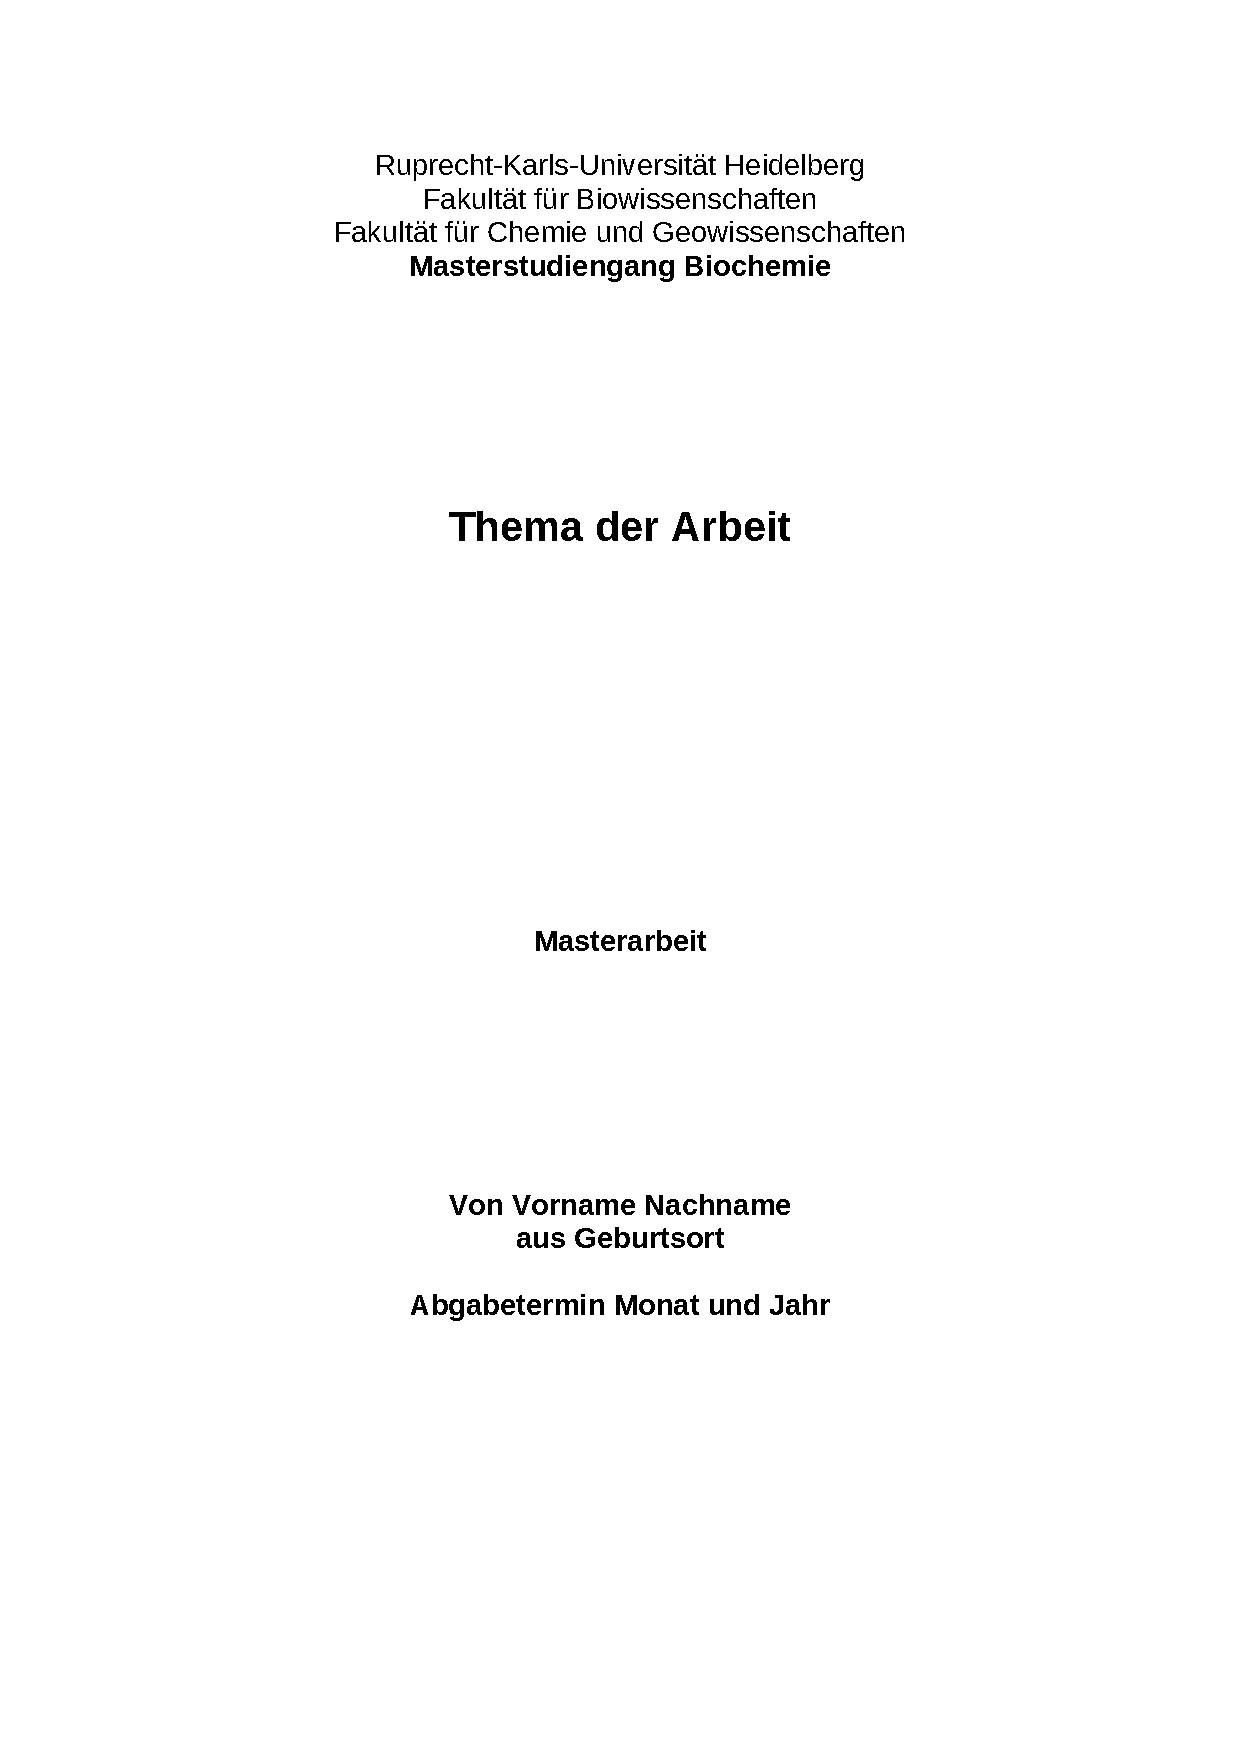
\includepdf[pages={1,2,3}]{sections/A-front-matter.pdf}

% odd pages at the beginning
\afterpage{\blankpage}

\begin{abstract}{english}
    English abstract.
\end{abstract}


\begin{abstract}{german}
    Deutsche Zusammenfassung
\end{abstract}

% You need to switch back to english at the end if you use a different
% langugate
\selectlanguage{english}
\afterpage{\blankpage}
\clearpage 

\section*{Acknowledgements}
\afterpage{\blankpage}
\clearpage


% Table of contents/list of figures/list of tables
% You can customize the table of contents depth
% I prefer that only two levels are shown (X.Y.),
% but it can show up to 3 (X.Y.Z)
\setcounter{tocdepth}{2}
\tableofcontents

\clearpage
\listoffigures
\listoftables

\clearpage

\pagenumbering{arabic}

% Using \include will automatically clear the page and import the section on a new page 
% Using \input will append it directly to the end of the previous section
\section{Introduction}

A customizable LaTex template for dissertations in the natural sciences.\supercite{MScTemplate.2024}




\subsection{Aim of this study}
\section{Results and Discussion}
\section{Conclusion and Outlook}
\section{Methods}


\clearpage 

% Start appendix/Uppercase roman numerals
\pagenumbering{Roman}

\printbibliography

\end{document}
